\documentclass[../main/main.tex]{subfiles}

\newdate{date}{16}{04}{2020}

\begin{document}

\section{Lecture 16}
\displaydate{date}. Compiled:  \today. Alice.

\subsubsection{Slide 240}

\begin{figure}[h!]
\centering
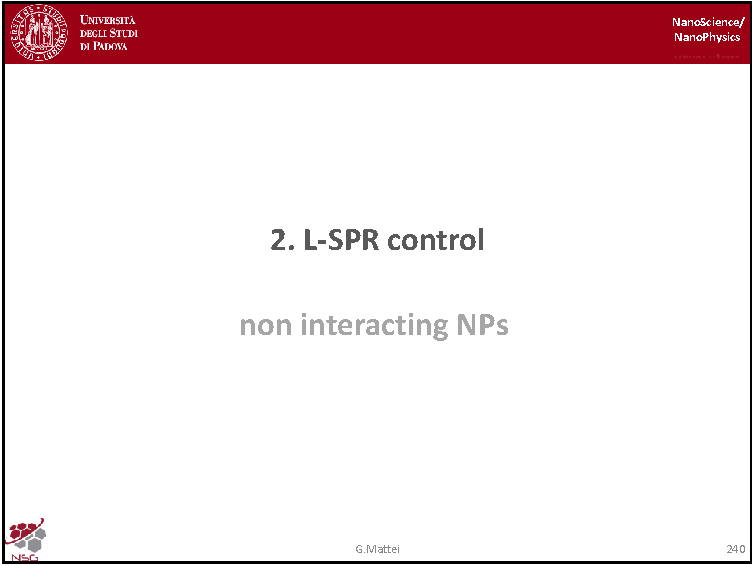
\includegraphics[page=1,width=0.9\textwidth]{../lessons/pdf_file/16_lesson.pdf}
\end{figure}

The two major achievement that we have done so far are:
\begin{itemize}
\item the capability to calculate the near and far field properties of an isolated nanoparticle in a non-absorbing medium trough the Mie theory.

\item the other important concept is the size dependent dielectric function, that we were able to obtain from the bulk dielectric function trough the semiclassical correction to the relaxation frequency in the Drude model.
\end{itemize}
These two pillars gives use the possibility to obtain full control of the spectral position of the localized surface plasmon resonance for non-interacting nanoparticles as we will see in the following.

This is important to discuss not only by itself, but also because when you want to deal with real world application or when you want to achieve specific funtionalitis out of your material, you need to design and control your nanosystem (or your nanomaterial) to do this job. For instance, when you want to obtain the SPR for a specific in a specific spectral position because your material, your application requires specific wavelength to operate with..or if your laser is tuned on tha specific wavelength, so that you need to know how to control those properties.
This would be the focus of this set of lessons.


\newpage

\subsubsection{Slide 241}

\begin{figure}[h!]
\centering
\includegraphics[page=2,width=0.9\textwidth]{../lessons/pdf_file/16_lesson.pdf}
\end{figure}

Of course the non-interacting case is just one of the possibilities that we have. Indeed, in this simple example we can see that if we look at this vials containing a solution of gold nanoparticles, the color of these solutions is due to different concentration of nanoparticles inside the solution.
This means you do not simply obtain a different intensity in the color, but real different colors. That is when you have interactions, that is when the nanoparticles are so close that the near field scattered dipolar-like field of one particles is affecting the near by nanoparticles. SO that, the incoming field is not only the plane wave that we shine, but also the plane wave plus the sum of all the scattered field from the other nanoparticles.
This is a clear example of interaction in a statistically defined sense. We will se how to deal with this aspect (figure d).


Another important point to deal with when you want to achieve specific funtionalities, is the shape of the nanoparticles.
Indeed, so far in the Mie theory we ere able to deal with spherical nanoparticles, but you can obtain different kind of shape. For instance in figure b we have nanoroads (road like nanoparticles) and if you change the aspect ratio (that is the ration between the length and the lateral size) you can control again the optical properties.
We will see how to deal with this kind of problems.


So let us try to focus first in the non-interacting case, to see which are the typical degree of freedom that we have to control the SPR position.

\newpage

\subsubsection{Slide 242}

\begin{figure}[h!]
\centering
\includegraphics[page=3,width=0.9\textwidth]{../lessons/pdf_file/16_lesson.pdf}
\end{figure}

To do this, let us look at this graph in which we compare nanoparticles with \( R=5nm \) embedded in silica but with different compositions (silver, gold and copper).

\begin{itemize}
\item As already discussed, the silver nanoparticles, since the threshold for inter-band transition occur more or less in the region between 300-400nm and the Frolich condition in silica is obtained at around 400nm that is quite far from that. In that case we have seen that the \( \varepsilon _2 \) value is sufficiently low to give a very sharp SPR resonance in silver.

\item On the contrary, if we look at gold, the Frolich condition in silica is obtained at around 530nm, but the threshold for inter-band transition occur exactly in that region, so there is a dumping of the coherence of the oscillation of the free electrons in the particles. In techniqual terms, the plasmon is said to decay into inter-band transitions, so the coherence of electrons which oscillates in phase is loss due to the onset of inter-band transition promoted from the \( d \) shell toward the \( s \) or \( p \) shells which are higher in energy.
So the region between 200 and 500nm is dominated by inter-band transition and you see that in the region of 200nm is of the same intensity of the SPR, so this means the relevance of the inter-band transition.

By the way, if you look at the value of the normalized extinction cross-section, you see that you obtained more or less one order of magnitude less intense interaction from silver with respect to gold.

\item The situation is even worst in the case of Copper. The SPR position (that is the Frolich condition) is obtained at around 570nm in silica, and the onset of the inter-band transition is even close to the 600nm in wavelength. So the resonance is even more dumped.

You can see that the absorbition around 200nm (which is triggered by the inter-band absorbition) is much more intense with respect to the SPR.

\end{itemize}
So normally copper is not considered a very good plasmonic material at least at the visible range, whereas gold probably is the best choice to do because of its chemical staibility more than for its intrinsic plasmonic properties.
But we will see that we can do better than this with gold in the following slide.

Of course, silver is probably the best in terms of the plasmonic properties because it behaves more closely to a real Drude metal, which is a metal in which no inter-band transitions are going on and so just free electrons operate and control the resonance.


In the plots on the right I reported a comparios between not only monoelemental systems made of gold and silver, but also an alloyed system, for instance an alloyed of gold ans silver togheter. On the top we have the simulation, while on the bottom the experiment. We did the simulation for a suitable model for alloyed dieletric function (non trivial object to obtain).

The most important message that I would like to give you in this example (right plots) is the fact that we can control the position of the localized surface plasmon resonance by controlling the composition of our material. So that we can do what is called the plasmon tuning, that is the tuning of the surface plasmon resonance as a function of the composition of our materials as we have seen in this experimental sample here.

This is of paramount importance when you want to obtain a tuning of your material to a specific external wavelength of your laser because your setup is tuned to work at that specific wavelength, and you want to achieve the resonance at that specific wavelength because at that wavelength some important things may happen.
So we need to know how to control the spectral position to obtain such kind of tuning in our system. The composition is one of the degree of freedom that we have to achieve this. Of course, we can do the very same plasmon tuning also if we are able to make an alloy of gold and copper, so we can tune in the rage between 530-570nm.

So globally we can go from 400nm up to 600nm just changing the composition of our nanoparticles if we want to tune the resonance in that specific range.
Of course, the composition probably is not the simplest way to tune the resonance, because it is not always possible to obtain an alloyed system. For instance, it is not straightforward to obtain a silver-copper alloy. You may remember that in the \emph{looster dishes}, there is no gold and you have just a combination of silver and copper nanoclusters in a given ratio to control the global color of that specific decoration.

But of course, controlling composition is a very clever way to obtain plasmon tuning and normally in all the technological applications alloyed systems performed better than monoelemental one because it can combine different properties in the alloy.

\newpage

\subsubsection{Slide 243}

\begin{figure}[h!]
\centering
\includegraphics[page=4,width=0.9\textwidth]{../lessons/pdf_file/16_lesson.pdf}
\end{figure}

Let us see for a given composition, the effect of size. The size is the other important degree of freedom that we have. Let us see how far we can go with the SPR control.

So far we have seen that changing the size, at least in a small range, does not produce large variations in the SPR position. That is because the SPR is controlled mainly by the Frolich condition if we are working under the dipolar approximation. The position of the resonance is given by the Frolich condition, whereas the width of the resonance is controlled by the value of \( \varepsilon _2 \) at that specific value of the wavelength.

I would like just to underline this result for \( R=1nm \) radius, that is a very very small radius for the gold nanoparticle in silica. You may see that the resonance is more or less in the same position, but there is this large tail toward larger wavelength. This is a warning message that we have from this extreme application of our size corrected dieletric function. To model all those samples (for the varius value of \( R \)) we need to use a size dependent dielectric function \( \varepsilon = \varepsilon (\omega ,R) \). You are seen that the Frolich condition for \( R=1nm \) is obtained at larger wavelength, so the message here is that the Frolich condition is one of the rules to predict the position. In particular, it is the most important one when the value of the \( \varepsilon _2 \) is not that large, but when \( \varepsilon _2 \) is very large of course at the denominator of the Mie extinction cross-section, it tends to dominate the two contributions (the one from the Frolich condition and the other from the \( \varepsilon _2 \)). So it is a trade-off between these two terms which controls the real or the apparent position of the resonance, because in this case the Frolich condition and the wavelength at which the \( \varepsilon_2 \) is slower, are no longer allined, so that we have a sort of distorted peak instead of a well-defined peak like in the other cases.

The other point that I would like to underline is the fact that for \( R=20nm \) we can clearly see that there is a slight red-shift of the position of the resonance. This is another indication that we need to work beyond the dipolar approximation, that is the \( l=1 \) expansion is no longer sufficient to describe the nature of our systems. So we need to resort to higher multipolarity and \( l=2,3 \) are tipical value that we need to have. These values may distort the global spectrum and tends to produce red-shift resonances.

\newpage

\subsubsection{Slide 244}

\begin{figure}[h!]
\centering
\includegraphics[page=5,width=0.9\textwidth]{../lessons/pdf_file/16_lesson.pdf}
\end{figure}

If we look at the very same graph but plotted in terms of the extinction efficiencies (that is the adimensional prameter, the cross-section normalized by the projected area of the particles). You can clearly see the very different extinction efficiencies of particles with different size.
But of course this is another way to recast the very same information that we had in the previous slide.

Here, we can better appreciate the fact that to obtain a better extinction efficience with respect to the pure geometrical one (that is \( Q_{ext}=1 \)) we need to work with a radius of around \( R=10nm \) or above. So that we can obtain better efficiencies in terms of the scattering and absorbtion cross-section.
This is of course in the far-field.

\newpage

\subsubsection{Slide 245}

\begin{figure}[h!]
\centering
\includegraphics[page=6,width=0.9\textwidth]{../lessons/pdf_file/16_lesson.pdf}
\end{figure}

If we look at the very same set of samples (so gold nanoparticles in silica), but now we increase the size well above the \( R=10nm \) in which we are expecting to go ok with the dipolar approximation. We need to resort to the fully multipolar expansion and we see that the effect is to produce a red-shift of this peak here (which is the dipolar resonance) and now we have the onset of the other additional resonances (quadrupolar and octupolar).
So this is a clear indication that we can no longer predict the position of the dipolar resonance with the simple Frolich condition because now the global resonance of the peak of the spectrum is controlled by different multipolar contribution, so we need to see the degree of resonances of the different Mie coefficients (\( a_l \) and \( b_l \)) in the cross-section, and so they can produce  resonances in different spectral region with respect to the simple dipolar one case (which is the one with \( R=10nm \)).

\newpage

\subsubsection{Slide 246}

\begin{figure}[h!]
\centering
\includegraphics[page=7,width=0.9\textwidth]{../lessons/pdf_file/16_lesson.pdf}
\end{figure}

As we can better see, for instance in the case of the efficiencies, also in this case of course when the size of the particle is larger, the extinction efficienciencies increases with the size. The maximum is for \( R=50nm \) and then it decreases, but with a broader features. So you may take advantage of all those resonances according to specific application you may need in your system.

\newpage
\subsubsection{Slide 247}

\begin{figure}[h!]
\centering
\includegraphics[page=8,width=0.9\textwidth]{../lessons/pdf_file/16_lesson.pdf}
\end{figure}

If we look at the case of silver, the situation goes more or less in the same way, apart from the fact that the resonances are sharper in this case.
As you can see, from \( R=1nm \) broader resonances (R=2,5,10,20,30,50nm) and in the case \( R=50 nm \) you are able of course to obtain the dipolar, quadrupolar and octupolar resonances.
This is a clear indication that the general rules that you may use to interpret the spectrum is that the dipolar resonance in the non-interacting case is the less energetic one, indeed is the one which occurs at larger wavelength because for larger wavelength the ration between size and wavelength is in favour of the dipolar approximation. That is the larger the wavelength, the better is the assumption that the field is constant all over the volume of the particle is better fullfilled.

\newpage

\subsubsection{Slide 248}

\begin{figure}[h!]
\centering
\includegraphics[page=9,width=0.9\textwidth]{../lessons/pdf_file/16_lesson.pdf}
\end{figure}

The other important degree of freedom that we have to control the SPR resonance is the matrix. If we take the very same nanoparticle, but with put it in different environment we can obtain dramatically different spectra.

This is the depicted in this simulation in which we have the extinction cross-section of a gold nanoclusters with radius \( R=2.5nm \) and embedded in different matrices, from silica up to titania (in the ??rootail?? configuration). So we have basically a variation of the refractive index (which is the square root of the \( \varepsilon _m \)) from 1.46 up to around 2.7 for the ??root tail?? titania.

You can clearly see that in this case even gold is able to produce a very nice resonace out of the very same size. Why this effect here?
This is why the Frolich condition (we are clearly in the dipolar approximation for so small size of \( R=2.5nm \)) for the case of \( n=2.7 \) is so far from the inter-band transition level which are uneffected by the matrix or by the size, so they are more or less here.

So in that case you can produce very larger resonances more or less as in the case of silver. So this is a very interesting message that we can give: so that the SPR is not an intrinsic property of that material (that is of gold), but is a combination of gold and the matrix.
So that we can obtain a better decoupling between the SPR resonance and the inter-band transition, so that you can improve the quality of the near field interaction in our system.
So from this the better dieletric properties of our composed (or meta material). We can speak about meta material because we can obtain novel functionalities by combining properties of different materials in site.

The other important result contained in this graph here is the fact that our nanoparticles are very sensitive to the dielectric environment in which they are embedded. This property can be used in a clever way as we will see in a moment, as optical sensors. That is we can obtain a very sensitive optical sensors from a nanoparticle which can tell us, with a simple extinction measurement, what is the dielectric function of the medium around its surface.
How can we do that? If we plot for instance the position of the SPR (as in this case) as the function of the refractive index we obtain the following graph (next slide).

\newpage

\subsubsection{Slide 249}

\begin{figure}[h!]
\centering
\includegraphics[page=10,width=0.9\textwidth]{../lessons/pdf_file/16_lesson.pdf}
\end{figure}

We have the position of the SPR as a function of the refractive index. We have a monotonic increase of that value, so that if we know the size of our nanoparticles, we can obtain information (measuring the position of the SPR) on the dielectric value of the refractive index in the matrix.

\newpage

\subsubsection{Slide 250}

\begin{figure}[h!]
\centering
\includegraphics[page=11,width=0.9\textwidth]{../lessons/pdf_file/16_lesson.pdf}
\end{figure}

Let us see for instance the very same effect for silver. Also for silver you can even improve the already sharp resonance for the silver nanoparticles in silica, by increasing the refractive index. The black curve is for \( n=1 \) (that is air or vacuum) and we end up with \( n=2.5 \). You see that we have:
\begin{itemize}
\item the red-shift. Why do we have the red-shift? Because if we go to the Frolich condition (we are in the dipolar regime), since the Frolich condition is fullfilled at much more negative value (because the \( -2 \varepsilon _m \) coefficient is more negative when the \( \varepsilon _m \) is larger) so that we need to move on the dielectric function the \( \varepsilon _1 \) of our particle which tends to \( - \infty  \) on increasing the wavelength, so that we need to move toward more negative values so we can need to move toward larger wavelengths.

So this clearly explain the position of the resonance, which is red-shiftted (this is very easy to be understood).

\item you have an increasing also in the intensity because of the better decoupling between the resonances and the inter-band transitions, and we are dealing also with region in which the \( \varepsilon _2 \) is slower. So that we can play with these three ingredients to obtain better resonances in our material.

\end{itemize}

\newpage

\subsubsection{Slide 251}

\begin{figure}[h!]
\centering
\includegraphics[page=12,width=0.9\textwidth]{../lessons/pdf_file/16_lesson.pdf}
\end{figure}

Also in this case, if we plot the SPR wavelength as a function of the refractive index we can have, in the left plot, a behavior which is better described by a parabola (it is not a linear fit) , so that we obtain the parameter in figure. SO that we can define what is called the \textbf{sensitivity} of our optical sensors: we can define what is the variation of the wavelength for a variation of the external refractive index. The larger is the value \( S_{bulk} = \pdv{\lambda _{SPR}}{n}  \), the better is the capability of our sensors in terms of the sensitivity.
Of course, if the curve is a parabola, it is first derivative with respect to the refractive index is a linear function, so we can obtain the value in the right figure.

 The quantity of \( S_{bulk} \) are (\( \lambda  \) is in nm, while n is an adimensional parameter but conventionally it is assigned to the RIU (refractive index unity) which is non normalized, but just to highlight that we have something which is the refractive index and to have a better remind that we are dealing with a variation of the refractive index). So when we are speaking about sensitivity we talk about \( nm/RIU \). We labeld the sensitivity as the bulk sensitivity because we are changin the bulk volume of the refractive index around the nanoparticle.

SO this plot here means that if you change for instance your refractive index, let us say from the one of silica to the one of titania, you can have a shift in the SPR which is of 140nm minus 100nm. So the relative shift is of 40nm, which is a remarkable quantity and very easy to be measured.
So for this reason, metallic nanoparticles gained a lot of interest for optical bionsensors. In our group we are investigating very intensively the use of those nanoparticles for bionsensors for achieve sensing with a molecules which can be attached to the surface.

The trick to obtain a molecular sensors (and not a bulk sensors) is to see which is the sensitivity not to a change of the global envoronment around the nanoparticle, but just a tiny layer around the particle is decorated with the molecule which you want to probe and this case you can obtain a local variation of the dielectric coupling and so we need to know how to handle with this particular situation. We will see this when we will discuss in a moment the core-shell situation.


\newpage

\subsubsection{Slide 252}

\begin{figure}[h!]
\centering
\includegraphics[page=13,width=0.9\textwidth]{../lessons/pdf_file/16_lesson.pdf}
\end{figure}

Another important effect that we need to take into account to control the spectral position of the localized SPR, is the shape.

Spherical shape is the most stable in terms of thermodynamics and any shape is converted to the spherical one if you increase the temperature, because thermodynamic ultimately wants to produce the lower surface with the very same volume and the sphere fullfill this requirement.

You know, the Mie theory is particularly suitable for spherical clusters, in the formula is ulltrstated the dipolar extinction cross-section.

Of course, you need to work with isolated non-interacting nanoparticles, with spherical clusters and non-absorbing medium and you need to know the dielectric properties of our materials.

How can we go beyond the MIe theory, is we have for instance an elgongated nanoparticle or an ellipsoidal cluster?


\newpage

\subsubsection{Slide 253}

\begin{figure}[h!]
\centering
\includegraphics[page=14,width=0.9\textwidth]{../lessons/pdf_file/16_lesson.pdf}
\end{figure}

We can use the \textbf{Gans Theory}. This theory is obtained by calculating the dipolar scattering from non-interacting volumes of materials and I will not enter into details of this theory.

We have the representation of the extinction cross-section of an ensamble of ellipsoidal particles with random orientation one with respect to the other, so that we can recognize a shape with this form of this equation which looks like very similar to the dipolar Mie one.
But we have now a summation over three elements \( j=1,2,3 \), which are not multipolar expansion, but just the fact that for non symmetrically ellipsoidal particle we have three axis (\( a_1,a_2,a_3 \)) and so they are different in principle (or they can be degenerate if the ellipsoid is prolate or oblate). But in general we need to define those three coefficients \( L_j \), which are the \textbf{polarization coefficients}, which are a geometrical adimensional quantities which describes the geometry of our system. They have a close relationship that is:
\begin{equation*}
  L_1 + L_2 + L_3 =1
\end{equation*}
and of course when the ellipsoid is fully degenerate (so it is a sphere), the three \( L_j \) should be equal so \( L_j = 1/3 \). If you substitute \( L_j = 1/3 \) in the previous cross-section formula, you will recover the full Mie formula for the resonances.

In the formula for \( L_j \), the parameter is \( e \) that is the \textbf{eccentricity}  of our system, which is defined by, if you for instance have a prolate ellipsoid (with \( a_1>a_2=a_3 \)), the formula
\begin{equation*}
  e = \sqrt{1 - \qty(\frac{a_2}{a_1})^2 }
\end{equation*}
For a sphere we have \( e=0 \).

I will not enter into many details here, but the most important message is that:
\begin{itemize}
\item  we have now a slightly different formula for the extinction cross-section with respect to the Mie case, in which we had \( 2 \varepsilon _m \), instead here we have the ratio \( \varepsilon _m (1-L_j)/L_j \), which is a generalized Frolich condition, controlled by the \( L_1,L_2  \) and \( L_3 \) coefficients.

\item The other imporant message is that instead of a single resonance, now we have three resonances, because in principle, since the \( L_j \) coefficient are different, we can have up to three different resonances. Of course if we look at the prolate ellipsoid like in this case, the two of those resonances are degenerate (because \( a_2=a_3 \)) and we have another resonance for \( a_1 \).
\end{itemize}
I would like to furtherly strees that this formula for the extinction cross-section holds for a random distribution of orientation of the ellipsoid with respect to the incoming plane wave.

Let us see what is the effect in terms of the cross-section of the Gans theory.


\newpage

\subsubsection{Slide 254}

\begin{figure}[h!]
\centering
\includegraphics[page=15,width=0.9\textwidth]{../lessons/pdf_file/16_lesson.pdf}
\end{figure}


The results are reported here.

\begin{itemize}
\item If we start from \( e=0 \) (perfect sphere), we have the standard resonance of gold nanosphere in silica.
\item Then if we go with larger eccentrities, for \( e=0.66,0.8,0.87,0.94 \) we see that we have the appearence of a distorted spectrum, which starts to exhibit a separation of the original resonance into two resonances as expected from the Gans theory, which we can interpret in the sense of different contribution on the previous formula that we have seen in the previous slide.
\end{itemize}
Here, we are just elongating the particle keeping constant \( b \equiv a_2 \) and \( c \equiv a_3 \) of 3nm. We move the major axis of our ellipsoid from 3 up to 9.
We can see that we can obtain very well defined resonances for all the elliposidal nanoparticles. we need now to unsterstand what is the nature of these two resonances.

For instance let us look at the red curve here, and compare it with the purple curve (for the sphere):
\begin{itemize}
\item we can easily recognize that the first peak is on the very same spectral position. This means that this resonance (1) is controlled by a size which is similar to the sphere. This means that we can interpret this resonance as the one occurring when the external dielectric field oscillates in the vertical direction (2) (for the sphere) or in the vertical direction (3) for the elliposid, because the effective size seen by the electric field is the very same as the sphere. Indeed, the spectral position does not change in this case.

\item whereas when we look at the other resonance, we can interpret that resonance (4) as the resonance occurring when the electric field oscillates in the horizontal direction.
\end{itemize}
This is consistent with the thinghs that we have understood from the previous slides, that is the effect of the size: the larger is the size, the red-shiftted is the resonace. This is a things that we can easily understand in terms of the things that we learned from the spheres.

But in this case of course, since we have a random distribution of the resonances, we just have two resonances, that is the longitudinal and the lateral kind of resonances.

Of course, if we would have not randomly oriented roads, but a well oriented roads (like in the samples that we have seen) which can be obtained by ion irradiation, or we can elongate the particles along the ion track in our system:
\begin{itemize}
\item of course if we shine light perpendicular to the samples, we just see one resonance, which is the first (1) because of course the apparent size that light see when enters perpendicular to the sample is the spherical section of the elliposid.
\item Whereas if we would enter laterally in the sample, light will see the elongated particles and we will see just the second resonance (with larger wavelength resonance (4)) which is controlled by the longitudinal resonance in our sample.
\item Of course we can obtain a combination of the two if we enter with the ??tilted?? illumination. So we can control at the level of behavior of our system, which is the sort of a ??DeCroix??  or birefringent system, because the property of refraction of ligth depends on the relative orientation of the light with respect to a given symmetry in our system.
\end{itemize}
 This is a very interesting application of the samples that we have seen obtained with these elongated nanoparticles. So we can obtain a birefringent system with a very simple technique.

\newpage

\subsubsection{Slide 255}

\begin{figure}[h!]
\centering
\includegraphics[page=16,width=0.9\textwidth]{../lessons/pdf_file/16_lesson.pdf}
\end{figure}

Another important shape that I would like to discuss is the \textbf{core-shell} geometry that we described before. The core-shell nanoparticle is composed by a core of radius \( R \) and dielectric function \( \varepsilon _c \) surrounded by a shell with thickness \( d \) of a material with dielectric function \( \varepsilon _s \). The core-shell is sorrounded by a medium with dielectric function \( \varepsilon _m \). Also in this case we assume \( \varepsilon _m \) as a real quantity, so the medium is not-absorbtion. But we let \( \varepsilon _c \) and \( \varepsilon _s \) be complex functions of the frequency (or of the wavelength).

This geometry here is very interesting for achieve a lot of different functionalities, and we will see how to obtain an optical molecular sensor out of this simple shape here.

In this case we can obtain the quantitative description of this geometry here, by a straightforward extension of the Mie theory.
We can obtain the very same expansion of the external incoming beam (the plane wave), but in this case we need to calculate additional fields: that is we need to calculate the fields inside the core  (electric and magnetic) and the fields inside the shell (electric and magnetic) and the fiels outside.
So basically we need to add a new set of coefficients of the multipolar expansion, and we need to solve the Helmholtz equations in spherical harmonics in all the core, the shell and the medium and to give the continuity equations in the three materials, so we can calculate the coefficients.
But now we have an additional interface between the core and the shell and from the shell with respect to the medium.


The theory is conceptually simple and there is a straightforward extension to multi-layered nanoparticles, that is multi-layered particles which is composed by core sorrounded by different levels of layers. We can obtain a closed solution of the fiels, so the solution is very simple.
But in terms for instance of the dipolar approximation, we can obtain a closed expression for the extinction cross-section, by looking at a very general expression that we have obtained from the Mie theory related to the imaginary part of the polarizability.

In this case, the polarizability is a little bit more complicated with respect to the simple expression that we gave for the dipolar approximation of the Mie theory and it is a very compact function of the dielectric functions of the shell, the medium, the core. In particular, we have the ratio \( \qty(\frac{R}{R+d})^3  \), which is the ratio between the inner core with respect to the outer global size of the shell (that is the radius+thickness of the shell), it is the relative fraction of the core with respect to the entire volume of the particles.

In the case of a single-core nanoparticle (if the thickness of the shell goes to zero), we can recover the Mie formula if we put:
\begin{equation*}
  \begin{cases}
   \varepsilon _s = \varepsilon _c\\
   R' = R+d
  \end{cases}
\end{equation*}
this is a degenerate case in which we have a mono compositional nanoparticle.

So the effect of the core-shell is the fact that you can modulate the properties of the core by addition of this dielectric function (the shell). So you can obtain really very interesting effect as we will see in a moment.

\newpage

\subsubsection{Slide 256}

\begin{figure}[h!]
\centering
\includegraphics[page=17,width=0.9\textwidth]{../lessons/pdf_file/16_lesson.pdf}
\end{figure}

Before discussing the application of these things, I would like to underline you a very very interesting concept.

If we were able to obtain a structure in which for instance we are able to control the dielectric properties of our shell, in principle we can ask the following question: is there a chance to modulate the properties of the shell so that we can make the polarizability \( \alpha =0 \)?

This is apperently a very simple question, but if you are able to do so (if \( \alpha =0 \)) at that specific value which fullfill this condition, the extinction cross-section goes exactly to 0. This means that basically we are no longer able to see the presence of the nanoparticles, because the plane wave arriving to the nanoparticle, for some magic trick, is uneffected (at that specific wavelength) by the presence of the nanoparticle. Normally, you see the presence of a particle because there is a distorsion in the otherwise homogeneous background of the external field. If you do not distort that background, either by absorbtion or by scattering, you cannot see anything in your material.

So the question is: are we able to obtain a core-shell system in which we are able to produce a 0 polarizability that is a 0 cross-section?
In that case we will not able to see the presence of the nanoparticle, as said. This problem is what is called the \textbf{invisibility cloak}, the fact that you can obtain in the Harry Potter way, you have a cloak around your nanoparticle so that you can stelp its presence with respect to an external observable, because your are able to switch off the absorbtion and scattering properties of the nanopartciles. So there is no distorsion of the external incoming wave in the far field so that you are not able to see the structure.

The possibility to obtain what is called invisibility, or invisibility cloak, is in our particular case controlled by the equation that \( \alpha =0 \), so that the numenator of the previous expression should go to zero, so that we obtain (1) (the core fraction is expressed as \( f \)).

So for any specific wavelength we can ask: is it possible at aptical frequency to achieve invisibility optical cloaking? which would be a very nice application of our theories.
We could obtain this invisibility if we are able to solve (1) for reasonable values of the shell material. That is: which is the composition of the shell so that we can obtain invisibility cloak for the core?

\newpage

\subsubsection{Slide 257}

\begin{figure}[h!]
\centering
\includegraphics[page=18,width=0.9\textwidth]{../lessons/pdf_file/16_lesson.pdf}
\end{figure}

Unfortunately, at optical frequencies this is not easily obtainable, because if we solve that equation (which is of seven order equation), for instance if we work with a core of gold like in this case, the dielectric function of gold are reproduced here. The black curve is the real part, the red curve is the imaginary part of the dielectric function. If we calculate the condition of cloaking, the shell should exhibit a dielectric function which reads as the blue curve (real part) and green curve (imaginary part):
\begin{itemize}
\item The problem is that the \( \varepsilon _2 \) of the shell (green) should be a negative value, which is not normally the case for standard materials because \( \varepsilon _2 \) is related to losses and have a negative losses means gain energies when you enter in a such material.
\item As far as the \( \varepsilon _1 \), it is reasonable, indeed it could be positive as the standard dielectric.
\end{itemize}
Hence, the major problem stands for the imaginary part which has to be a negative value.

This plot is for a particular value of the \( f \) (filling fraction of the core).

\newpage

\subsubsection{Slide 258}

\begin{figure}[h!]
\centering
\includegraphics[page=19,width=0.9\textwidth]{../lessons/pdf_file/16_lesson.pdf}
\end{figure}

We could see also other solutions. In this case, if we still zoom in the region near zero, we see that the results that we obtained in terms of the imaginary part of the other solution is a negative value.

\newpage

\subsubsection{Slide 259}

\begin{figure}[h!]
\centering
\includegraphics[page=20,width=0.9\textwidth]{../lessons/pdf_file/16_lesson.pdf}
\end{figure}

We can see the zoom of that region.
The negative value means that to achieve optical cloaking, the material of the shell is a non standard material, that is a material that we need to ingeener to obtain such a control of the cloaking possibilities. This has lot of applications: for instance if we were able to obtain such an invisibility cloak for microscopic oject, you could produce the real invisibility cloak, so you could stelp macroscopic object as well as nanoscopic objects. Of course, this is for the moment not possible, but we will see how to obtain something which is closely resemble at this effect at different frequency, when we will speak about negative refraction meta materials.

\newpage

\subsubsection{Slide 260}

\begin{figure}[h!]
\centering
\includegraphics[page=21,width=0.9\textwidth]{../lessons/pdf_file/16_lesson.pdf}
\end{figure}

For the moment I would like just to highlight this fancy properties and to stimulate your tought on this direction. There is a lot of people trying to investigate the invisibility cloak, which is represented here.

If you have a set of four nanoparticles, suitably coated with a material which fullfill the invisibility cloak for that particular system, you see that if you shine light coming from the right direction, the wavefront is locally distorted. But in the far field you see in the region (1) that you obtain a still plane wave, which is slightly distorted. So there is no distortion in the far field when you are looking in the material, so you can obtain meta material, which shadows your basically nanoparticles so you cannot see them.
You can achieve this by a clever engigneering of the optical properties of your cloaking.


\newpage

\subsubsection{Slide 261}

\begin{figure}[h!]
\centering
\includegraphics[page=22,width=0.9\textwidth]{../lessons/pdf_file/16_lesson.pdf}
\end{figure}

There is a very interesting and very hot research field in which the only ingredient that you need to put, for obtaining the cloaking, is to have a material wich exhibit gain to compensate the losses of your nanoparticles, as we have seen in the simulation.

If you have gain in the external field, you need to re-pump the energy which is loss by absorbtion and by scattering, so that you can re-build the decreasing in the intensity emerging from the nanoparticles without the cloaking. So you have the full reconstruction of the plane wave field, so that you can obtain the invisibility cloak as reported in this paper.

We are trying to work with the material working in this line (red line) and not exactly in the cloaking which has been demonstrated that in the visible range is very difficult to achieve.

In the concept of developing materials, with a clever or active properties (in the sense that they can compensate for loss and produce optical gain), indeed we are working in the field of nano lazying that is the production of gain medium at the nanoscale to produce coherent sources of light with nanometric size.

\newpage

\subsubsection{Slide 262}

\begin{figure}[h!]
\centering
\includegraphics[page=23,width=0.9\textwidth]{../lessons/pdf_file/16_lesson.pdf}
\end{figure}

If you now get back to a more standard kind of core-shell system, in which we have a plasmonic core (that is a silver nanoparticle) sorrounded by a shell with purely real dielectric function (that is dielectric material), or embedded for instance in air or other inveronments. We can obtain out of this very simple system and interesting biosensors, indeed if we decorate the surface with an increasing thickness layer of given refractive index, for instance of n=1.5 (which is the typical refractive index of molecular systems), we can obtain a very interesting red-shift as a function of the shell thickness (when the shell thickness goes up to 10nm in thickness).


\newpage

\subsubsection{Slide 263}

\begin{figure}[h!]
\centering
\includegraphics[page=24,width=0.9\textwidth]{../lessons/pdf_file/16_lesson.pdf}
\end{figure}

If we plot the position of the surface plasmon resonance as a function of the shell thickness, in this case we have a curve like the one on the left, which can be fitted by a curve with evolution:
\begin{equation*}
  \lambda _{SPR} = \lambda _0 + A(1- e^{-t/\tau } )
\end{equation*}
which is a sort of an exponential evolution, which tends to saturate to an amplitude \( A \) which is the maximum excursion from 0 to the maximum thickness that we can obtain, starting from a given \( \lambda _0 \), which is the \( \lambda  \) whose SPR has zero thickness.

Of course, also in this case we can obtain a nice representation of this evolution in terms of sensitivity. In this case we can define what is the sensitivity of our nanosystem to this decoration with an increasing thickness of a given refractive index material.
So we can calculate, the \textbf{local sensitivity} (or surface sensitivity), which is defined in a similar manner as the bulk sensitivity. Indeed, we have what is the variation of the SPR position, with a variation of the thickness (t) for a given variation with respect to the ambient dielectric value \( \frac{1}{\Delta n} \) which is air. In this case, if we add a material which produces a jump in refractive index of \( \Delta n \) with respect to the external medium, we need to normalize for this variation the variation of the wavelength of the SPR.

In this case, we obtain also the derivative of the curve on the left, which is simply calculated by the expression:
\begin{equation*}
  S_{loc} = \frac{1}{\Delta n} \frac{A}{\tau } e^{-t/\tau }
\end{equation*}
and which is an exponential decay with an amplitude which is controlled by the \( \frac{1}{\Delta n} \).

The other important parameter in the fit is \( \tau  \). You may remember that \( \tau  \) is the \textbf{intrisinc scale} for the variation of the \( \lambda _{SPR} \). In this case, you see that \( \tau = 2.7 \pm 0.1 nm\), this is the decay length of the field ouside the nanoparticle. Indeed, why do we need to expect this exponential saturation of the sensitivity to the thickness (left plot)?
This is because when the near-field around the nanoparticle, which we have seen in the dipolar approximation, is the field of the dipole centered at the center of the nanoparticle, when this field is already decayed we are no longer able to fill the composition of the shell around the nanoparticle which is the core. That is when the thickness is sufficiently larger with respect to the intrisinc decay length in that specific medium, we lose sensitivity to the thickness. In this case, the nanoparticle thinks to be in an homogeneous environment with a new refractive index of \( n=1.5 \) which is the refractive index of the shell. So we need to expect this saturation with this simple argument. So we need to expect a decrease in the local sensitivity for larger thicknesses. Hence, the best sensitivity of course is achieved in the limit of thickness going to zero, because in that case we have the full local field which decays as the third power of the distance.

So in our system we see that the near field decay in few nanometer.
So if we are able to build a system which is able to change the dielectric property from 1 (the refractive index of air) to 1.5 (the refractive index of the material), and all the modulation in between, we are able to obtain a sensitivity to the decoration of our surface with suitable molecules.
So the larger is the concentration of molecules at the surface, the larger is the effective refractive index of our material. So that we have a larger dielectric variation, so that we need to expect (like in this case) a red-shift of the SPR. And the larger is the sensitivity, the better is our capability to detect smaller concentrations of the molecules that we want to detect. They could be the antigens produced by our body when a virus attack our system and all those kind of things. They could be immobilized with a suitable ??resector?? at the surface of our nanoparticles, so that we can obtain a very sensitive and specific sensors, which is able to detect just that specific molecule in a complex fluid and capture that and change the local dielectric field around the nanoparticle and obtain this very interesting sensing capability.

For instance, in this case, the units of the local sensitivity is \( 1/RIU \). We have 32 of local sensitivity for thickness going to zero, so if we are able to build a sensor which is able to decorate with a 3nm of thickness around the particle we are in the range of 12 for local sensitivity. So we can obtain a very nice local sensitivity which is able to spot even femto molar concentration of a given molecule in an external medium. We are working in our group intensively in this kind of field to produce even more effective biosensors for different diseases.


\begin{remark}
Hence, the larger is the concentration of molecules at the surface, the larger is the effective refractive index variation of our material, and the larger is the sensitivity, the better is the capability to detect a small concentration of molecules (this technique is used to detect antigens cells in the blood for example).
\end{remark}


\newpage

\subsubsection{Slide 268}

\begin{figure}[h!]
\centering
\includegraphics[page=25,width=0.9\textwidth]{../lessons/pdf_file/16_lesson.pdf}
\end{figure}

Another very important class of core-shell material is the reversal of the previous. In the previous we had a plasmonic core sorrounded by the dielectric shell, while in this case we have a silica core (that is a dielectric core) and a metallic shell around sorrounded by water for instance. This particular system is called nano-shell, in the sense is a shell of plasmonic material decorating a dielectric sphere, so we have a metals sandwhiched in by two dielectris like in this case.
This is very interesting because it allows a good plasmon tuning, with a relative ease of fabrication. It is not so straightforward, but it is very interesting to work with this kind of system.
Of course we have the multilayered Mie theory which is able to provide us how to calculate the optical properties of this system.

Of course if the layer has for instance a finite core of \( R=60nm \) of silica, if we had an increasing amount of gold on top, we can very simply obtain a large shift in the resonance. We have a beautiful resonance for \( 5nm \) (it is very intense because it is decoupled from the inter-band transition of gold, as we have already underlined). Moreover, for the balck curve we have also a multipolar resonance.

The most important thing is that we can play with the position of this resonance by adding tiny amount of metals. Of course, it is not that straightforward to obtain this system, we worked with a modified version of this nano-shell working with a semi-nano-shell that is a core of silica partially filled (just in one side) so that we have an asymmetry in the dielectric properties (and in the plasmonic properties) and we can obtain very nice properties for biosensors and ??nanolazing??.

Just to stay on a very basic description of this system, if we add an increasing amount of gold, for \( 40nm \) of thick of the shell, we more or less are get back in a situation in which we are no longer sensitive to the presence of the dielectric core and we get an extinction cross-section which closely resemble of that of a nanoparticle made out of gold with a global size of 100nm (60+40nm).
This is because those quantities are controlled to a large extent by the most external layer in our multi-layered nanoparticle. Since the external field is not able to enter within the metallic nanostructure, it is not able to fill which is the composition of the core, because it is extinguished by the metallic thickness. So it is another way to re-think about the nature of the interaction between an electric field and a metallic nanoparticle, in which just for the dipolar case we are able to fill a constant field inside the material. But for a multipolar expansion we have seen that the field inside the nanoparticle is no longer constant and it is just confined on the outer surface of the material.

So with a conceptually very simple system, in this case we can tune very easily the resonance in region which are very interesting for application in biological systems. Our body has a maximum trasparency where water has the maximum transparency, that is in the region from around 900nm.
In the nearly infrared (from 800nm up to 1000nm), you have the best trasparency. Indeed, when you illuminate thinner part of your finger, for instance you just see the red light component, that means it is the less absorbed with respect to the spectrum. So that when we want to obtain systems that we want to illuminate from outside, or that we want to emit light from the inside toward outside our body, the window of maximum trasparency is very important. So it is important that you have resonances in the range between 800nm-1000nm. So if you are able to control the thickness of the gold shell, we can obtain straightforwardly this property.

The nano-shell were able to obtain very nice target in system, that is they can address those particles by proper functionalization toward tumoral cells, so this nanoparticle is able to selectively attach to tumoral cells, so that we can shine light from outside. The electron in the shell are able to resonate, so they dissipate energy, so they will hit up with this standard Joule effect, so that you can hit up those nanoparticles locally, just where the reached the tumoral cells. So you can do iperthermia in the body just using those clever targeting agent, so that you can obtain local hiting (there is no need to reach very high temperatures, something above 42-43 degree is sufficient to burn the cells, because it denaturates the DNA of that cells and stopping the reproducing of the virus and so on and so forth). For that reason it is a very clever system to work with. For us the main point is how we can control it, so how we can do the plasmon tuning to obtain the resonance exactly where we want to have. We are most interested in how we can control the optical properties, but of course those things have a large variety of applications.

\newpage

\subsubsection{Slide 269}

\begin{figure}[h!]
\centering
\includegraphics[page=26,width=0.9\textwidth]{../lessons/pdf_file/16_lesson.pdf}
\end{figure}

In thi case we have the effect of chaning the thickness of the core for a given shell thickness. If we change the dielectric core diameter, we can obtain a large tuning of the resonances as we have shown here. It is of course because the multipolar nature, even if the thickness is so small, but since the global size of the shell is very large with respect to the wavelength, we have to expect multipolar resonances. Indeed, it is what we have obtained as a function of the core radius with this very large tunability in the system.
So this is  a very clever system to obtain plasmon tuning.

\newpage

\subsubsection{Slide 270}

\begin{figure}[h!]
\centering
\includegraphics[page=27,width=0.9\textwidth]{../lessons/pdf_file/16_lesson.pdf}
\end{figure}

The other major point that we have so far neglected is the fact that in a real world application we do not work with monodispersed systems. So far we spoke about nanoparticles with a given size and we have assumed that all the particles are similar. But as we have seen in real samples, we have a size distribution: how can we handle samples with the size distribution? And how can we obtain informations from the optical spectra on the size distribution of the system?

This is a very difficult problem to deal with. In general, obtaining informations on the size distribution from the optical spectra is a very difficult task. It is becausde either we have a large distribution or it is really very difficult.
This can be seen on a very general framework as we will see in a moment.

\newpage

\subsubsection{Slide 271}

\begin{figure}[h!]
\centering
\includegraphics[page=28,width=0.9\textwidth]{../lessons/pdf_file/16_lesson.pdf}
\end{figure}

In general, the direct problem if we have a given size distribution (that we know) and we want to compute the extinction cross-section of our system (that we can obtain from a Lambert-Beer measurements, \( I(x) = I_0 e^{- \gamma x }  \)), normally we can define for our system the extinction coefficient \( \gamma   \) which is the concentration of nanoparticles times the cross-section for those nanoparticles. But of course if instead of having a monodispersed system, we have a given size distribution function \( f(R) \), which we will assume it is a normalized function (that is for the radius ranging from 0 to infinity, the integral of the distribution function is 1), we can build the equivalent of the extinction coefficient \( \gamma (\omega )  \) by integrating the size dependent cross-section weighted by the size distribution function and multiplied by the global concentration of nanoparticle for the entire volume:
\begin{equation*}
  \gamma (\omega ) = n \int_{0 }^{\infty } \sigma _{ext} (\omega ,R) f(R)\dd[]{R}
\end{equation*}
SO this is a straightforward generalize of the simple formula of before. Indeed, we can recover the previous formula \( \gamma (\omega ) = n \sigma _{ext} (\omega )  \), if we consider for instance a monodispersed system in which the size distribution is a delta function peaked at the \( R=R_0 \) radius, that is the average radius that we are dealing with.

Normally, in reality with have different sizes distribution:
\begin{itemize}
\item the most intuitive could be Gaussian one.
\item as we have seen, in real world applications, thermodynamics tells us that we better have to work with a log-normal size distribution as we have seen in real samples. We have a modified version of the standard gaussian in which all the variables are logarithm of the size, and we have also the \( 1/R \) coefficients which is the change of variable when we change from linear to logaritmic variable in the gaussian distribution.
\end{itemize}
In the plot we compare the delta function, with a gaussian distribution with the very same \( R_0 \) mean value and with a log-normal which is an asymmetric monomodal distribution with the very same average radius.


\newpage

\subsubsection{Slide 272}

\begin{figure}[h!]
\centering
\includegraphics[page=29,width=0.9\textwidth]{../lessons/pdf_file/16_lesson.pdf}
\end{figure}

What is the effect of size distributed system on the external measured optical properties?
We can see the effect of the size distribution on the optical properties in these plots here.
You mary remember that it is the sample with gold implanted nanoparticle in silica. As a function of the annealing time we have different sizes (left plot) and this is for instance an information that we have obtained by fitting for instance the spectrum obtained with the annealing for three hours (right plot). In the right plot, the solid line is the experimental optical properties and the dotted points are the Mie fit in this particular case (3h of annealing). The average diamater obtained by TEM was 5.3nm and the average diameter obtained by a fit is 5.2nm. Of course this level of agreement is very nice, but of course we are not able to obtain informations on the size distribution, which you may remember is very large in that case. In this case the size distribution is very large because at that time the Ostwald rippening was already effective and we were obtaining a very large size log-normal distribution.


\newpage

\subsubsection{Slide 273}

\begin{figure}[h!]
\centering
\includegraphics[page=30,width=0.9\textwidth]{../lessons/pdf_file/16_lesson.pdf}
\end{figure}

The relative lack of sensitivity of our measured optical spectrum to the size distribution, can be obtained in the reverse way.
If we calculate for instance the difference between a monodispersed system (red curve) with an average radius of 5 nm and the very same system (blue curve) with a size distribution of 2 nm (which is quite high).
Normally, we consider a system as monodispersed when the fullwidth divided by the average radius si less than \( 5\% \) ($\frac{FWHM}{R_0}<0.05$).
In this case we have around \( 40\% \), so it is definitely not monodispersed system.
But still the difference between a guassian distribution (1) and the monodispersed case can be negligible. So clearly we are not sensitive to this specific degree of freedom in our system.
So this is a warning message: if you want to extract information on the size distribution this will be a really thought job when you want to do in the reverse way, that is from the experimentally measured spectrum obtain something on the size distribution. So please, being carefull on doins such kind of things.

\begin{remark}
To summarize, if we want to obtain information about size distribution, we can not use such kind of optical measures.
\end{remark}



\clearpage



\end{document}
